%!TEX root = ../report.tex

\chapter{Convolutional Neural Networks and Semantic Segmentation}

	In this chapter, we look into the basic concepts of neural networks and later, how such concepts have been used for the task of semantic segmentation. In section \ref{section:ann} we present an overview of Artificial Neural Networks. In \ref{section:cnn} we look into basic concepts underlying Convolutional Neural Networks (CNNs). In \ref{section:cnnseg} we look into how CNNs are adapted for the task of semantic segmentation.

\section{Artificial Neural Networks}
\label{section:ann}

Artificial Neural Networks (ANN), inspired by the neural networks in our brain, was designed to learn tasks without explicitly programming descriptive features of the concerned tasks. An ANN is made up of processing units called neurons which performs a non-linear transformation, using an activation function, of the weighted linear combination of inputs. Figure \ref{Fig:haykin_ann_n} illustrates a non-linear model of a neuron. Many such neurons are connected to one another in an ANN resulting in its ability to learn highly non-linear function mappings from input to output space. Figure \ref{Fig:haykin_ann_ml} illustrates a multilayer feedforward neural network which is a type of ANN.

	\begin{figure}
		\centering
		\begin{subfigure}{.5\textwidth}
			\centering
			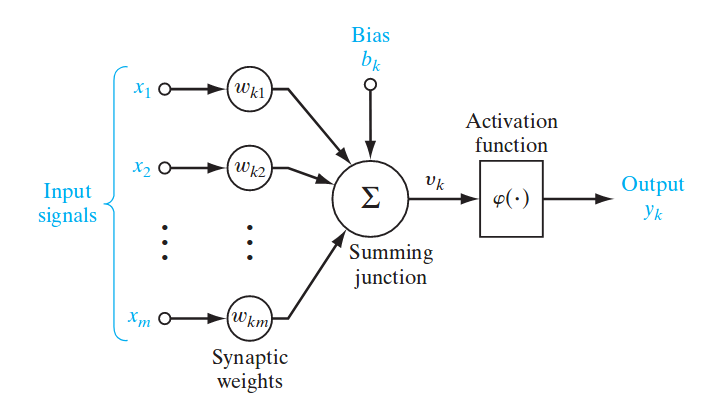
\includegraphics[width=1\linewidth]{images/neuron}
			\caption{}
			\label{Fig:haykin_ann_n}
		\end{subfigure}
		\begin{subfigure}{.3\textwidth}
			\centering
			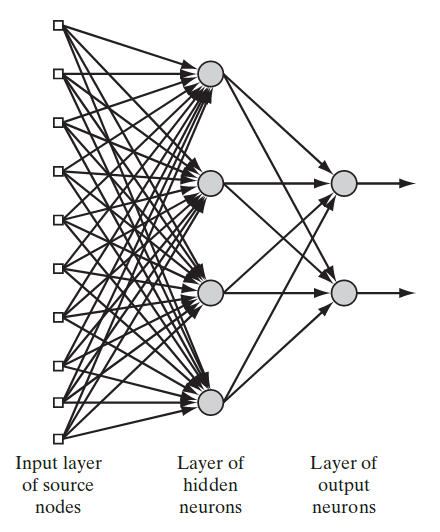
\includegraphics[width=1\linewidth]{images/ml_ff_nn}
			\caption{}
			\label{Fig:haykin_ann_ml}
		\end{subfigure}
		\caption{(a) A non-linear neuron model. $v_k$ = $\sum_{i=1}^{m} w_{ki} x_i$ denotes the local field of the neuron, $\varphi$ is the activation function and $y = \varphi(v_k)$ is the output of the neuron. (b) An illustration of a multilayer feedforward neural network with input source nodes, one hidden layer of neurons and an output layer of neurons \cite{haykin}.}
		\label{Fig:haykin_ann}
	\end{figure}

\section{Convolutional Neural Networks}
\label{section:cnn}

Convolutional Neural Networks (CNNs or Conv Nets) are a class of feedforward neural networks which are used in the field of computer vision. Tasks such as image classification, object detection, and semantic segmentation make use of CNNs. Unlike the multilayer feedforward neural network shown in Figure \ref{Fig:haykin_ann_ml}, CNNs are designed to handle image data which is usually represented as a stack of 2D values. A major part of CNNs comprise the use of convolutional layers which substantially reduce the number of parameters in comparison to fully-connected layers.

\subsection{CNN Architecture}

The general architecture of a CNN is illustrated in Figure \ref{Fig:cnn_arch}. A CNN is composed of different layer types such as convolutional layers, pooling layers and fully-connected layers. Each of the layers is looked into in detail in the subsequent sections.
	
	\begin{figure}[h]
		\centering
		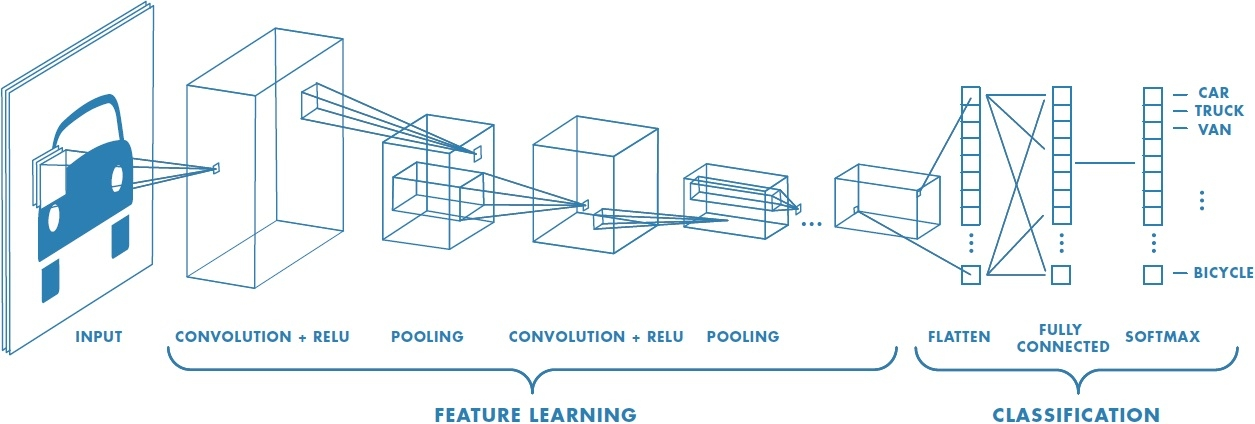
\includegraphics[width=1\linewidth]{images/cnn_matlab}
		\caption{This figure illustrates a CNN architecture. A convolution layer convolves on the input image or feature maps followed by an ReLU activation which produces output feature maps. A pooling layer downsamples feature maps. The CNN architecture shown, performs feature learning and classification \cite{matlab_cnn}.}
		\label{Fig:cnn_arch}
	\end{figure}

\subsubsection{Convolutional layer}

An RGB image typically consists of height, width and 3 channels representing red, blue and green. In order to better handle this structure of an input image, the neurons in a convolutional layer are arranged in a 3D volume of height, width, and depth. Each neuron is only connected to a small region in the input resulting in "local connectivity".  A hyperparameter called receptive field \cite{cs231n} controls the extent of the input region to which a neuron connects. An illustration of the 3D arrangement of neurons can be seen in Figure \ref{Fig:cnn_neuron}. When moving along the depth dimension, each 2D arrangement of values are called filters or kernels.

	\begin{figure}[h]
		\centering
		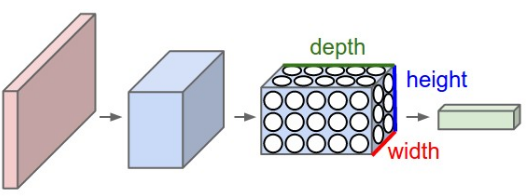
\includegraphics[width=.4\linewidth]{images/conv_3dneurons}
		\caption{Illustration of 3D (height, width, depth) arrangement of neurons in a convolutional layer. The convolutional layer transforms a 3D input volume to a 3D output volume  \cite{cs231n}.}
		\label{Fig:cnn_neuron}
	\end{figure}
	
A convolution filter slides through an input channel, performs convolution and produces output feature maps. A filter looks for specific features like edges and corners, at the input spatial location it convolves over. As an extension, a filter can be seen as a template image looking for a template across the input space. Figure \ref{Fig:convolution} illustrates one such filter which looks for vertical lines. 

	\begin{figure}[h]
		\centering
		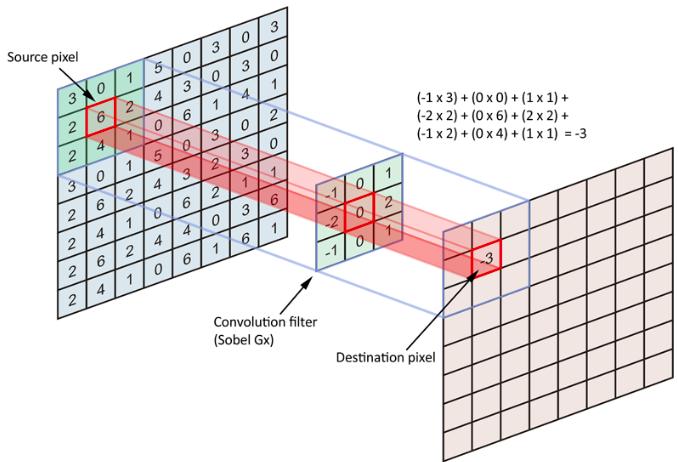
\includegraphics[width=.8\linewidth]{images/convolution}
		\caption{This figure shows a Sobel kernel convolving over an input. This kernel looks for vertical edges in the input image. The kernel values are multiplied elementwise with the input locations, and the results are added together to get the value at the location in the output feature map which corresponds to the center of the image locations  \cite{freecodecamp}.}
		\label{Fig:convolution}
	\end{figure}
	
The entire 3D convolution filter slides along the height and width of all channels of the input space looking for features along spatial locations and features across input channels. One 3D convolution filter results in a 2D feature map. Multiple such 3D convolutions are used each of which leads to a 2D feature maps which are all stacked along the depth dimension to create the output 3D volume. This process is illustrated in Figure \ref{Fig:3dconv}.

	\begin{figure}[h]
		\centering
		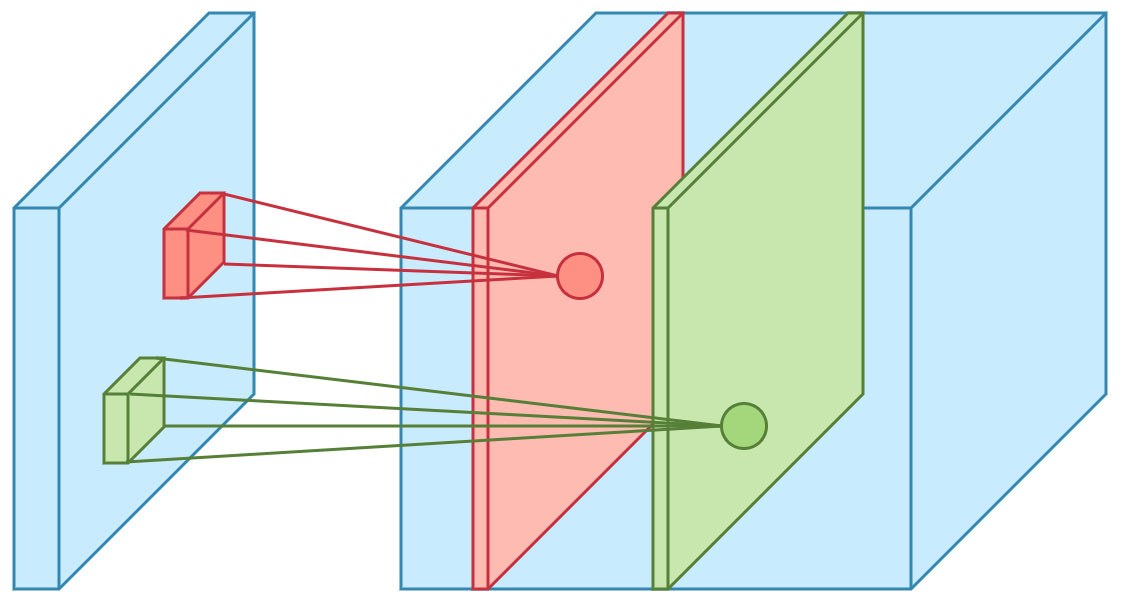
\includegraphics[width=.3\linewidth]{images/3d_conv}
		\caption{Illustration of 2D feature maps produced by two 3D convolution filters which are arranged along the depth dimension  \cite{towardsdatascience}.}
		\label{Fig:3dconv}
	\end{figure}
	
In CNNs, the filters are learned through training the CNN for a specific task such as image classification. Once a CNN is trained, the filters in the lower layers often tend to learn simple features such as edges and corners and filters in the higher layers learn more abstract features building upon the features learned by filters in the previous layer. 

	\begin{figure}[h]
		\centering
		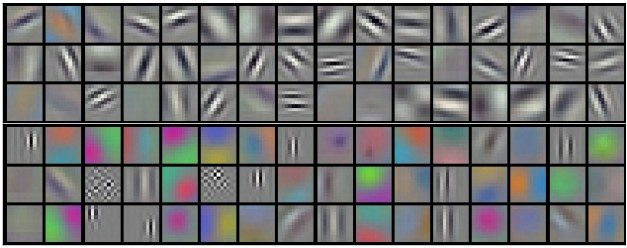
\includegraphics[width=.8\linewidth]{images/conv_template}
		\caption{Learned filters of AlexNet CNN architecture. The filters have learned to detect features such as lines, blobs and so on \cite{cs231n}.}
		\label{Fig:conv_template}
	\end{figure}
	

\subsubsection{Pooling layer}

A pooling layer is responsible for reducing the spatial size of the feature maps leading to a reduction in the number of trainable parameters in the network. This reduction in trainable parameters leads to reduced chances of overfitting and reduced computational cost. Additionally, pooling makes CNNs invariant to translations in the input image. This induced translation invariance is desired for tasks such as image classification where it is only required to find objects in an input space irrespective of where the object is located within the image. 

A pooling filter looks at a particular window in a depth slice (one 2D feature map out of 3D input feature maps) of input feature maps and produces one value as output for the window. Two common pooling types are max pooling and average pooling. The pooling filter outputs the maximum of all values and average of all values for max pooling and average pooling respectively. An illustration of max pooling and reduction in the spatial size of feature maps is shown in Figure \ref{Fig:pool}.

	\begin{figure}[h]
	\centering
		\begin{subfigure}{.35\textwidth}
  			\centering
  			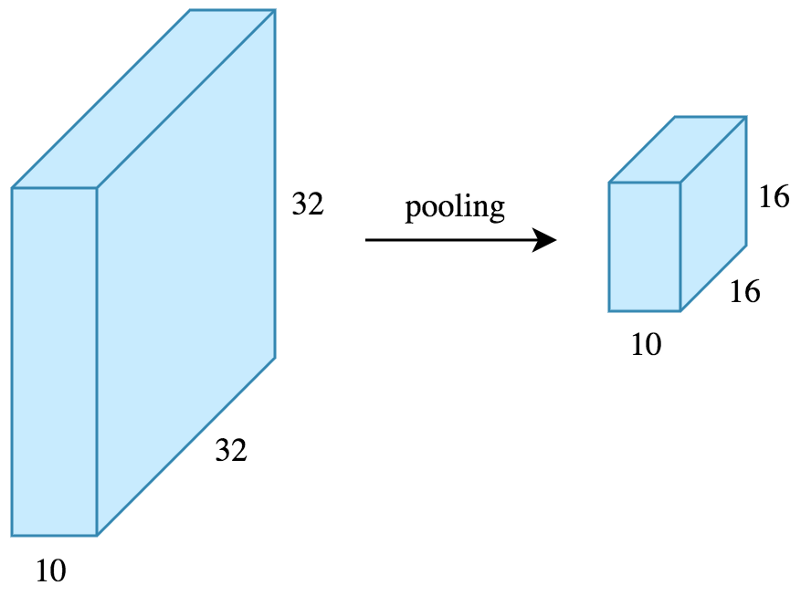
\includegraphics[width=1\linewidth]{images/pooling}
  			\caption{}
  			\label{Fig:poolb}
		\end{subfigure}
		\begin{subfigure}{.55\textwidth}
  			\centering
  			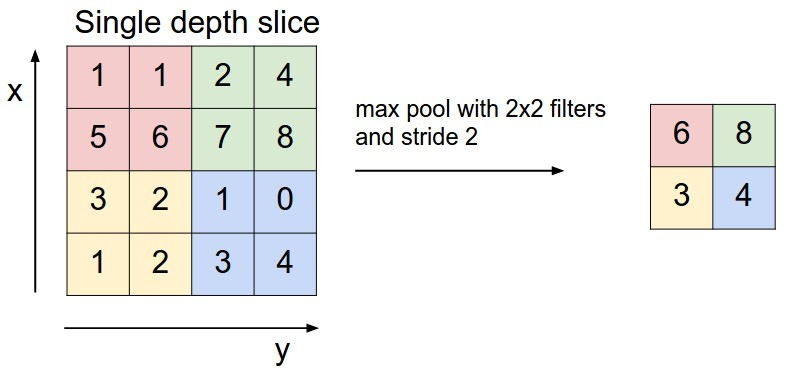
\includegraphics[width=1\linewidth]{images/maxpool}
  			\caption{}
  			\label{Fig:poola}
		\end{subfigure}
		\caption{(a) Illustration of feature maps being downsampled by pooling \cite{towardsdatascience}. (b) Illustration of max pooling where the pooling filter looks at 2$\times$2 input windows. Stride 2 denotes that the window moves two steps when it moves through x or y. Each color in the depth slice of input feature maps indicates a different input window and the corresponding color in the output feature map shows the selected max value \cite{cs231n}.}
		\label{Fig:pool}
	\end{figure}	


\subsubsection{Fully-connected layer}

In fully-connected layers, every neuron in a layer is connected to all neurons or input nodes in the previous layer. The hidden layer shown in Figure \ref{Fig:haykin_ann_ml} illustrates a fully-connected layer. In CNNs, the outputs produced by convolutional layers and pooling layers are 3D feature maps whereas a fully-connected layer expects a 1D vector as input. Therefore, 3D feature maps are converted to a 1D vector which is then given as input to fully-connected layers. There are two ways in which this 1D input to fully-connected layers is created in CNNs. One way is to flatten the 3D feature maps directly. For instance, if the 3D feature maps have a dimension of 7$\times$7$\times$5, the values are arranged in the form of a 1D vector with 245 values. In a second way, a technique called global average pooling is used to take the average value out of every depth slice of the 3D feature maps and then create a flattened 1D vector. If the feature map is of dimension 7$\times$7$\times$5, average value out of 5, 7$\times$7 depth slice is taken to get 1$\times$1$\times$5 feature maps. These feature maps are flattened to create a 1D vector input with 5 values as input to fully-connected layers. The output of fully-connected layers is then fed to a softmax function which converts the output into probability scores for the different classes involved.

\section{CNNs for Semantic Segmentation}
\label{section:cnnseg}

The CNN architecture discussed so far, learns to extract features and perform image classification by resulting in a probability score for each class. For instance, for a 10 class classification problem, for every input image, a trained CNN produces 10 values in the range [0,1] each of which provides the probability that the image belongs to the corresponding class. However, semantic segmentation is a dense prediction task which requires a class to be assigned to every pixel in the input image and hence for every input image, the output is expected to be another image of the same spatial size as the input image and contains in every pixel a value which denotes a class. This output is called a segmentation map. 

For this reason, two changes are done to the CNN architecture. One is replacing fully-connected layers with convolutional layers, and the other is upsampling the final feature maps produced back to the original input spatial size. Fully-connected layers require a flattened 1D input vector and produce a 1D vector as output. However, semantic segmentation requires a 2D segmentation map as output. Hence, fully-connected layers are replaced with convolutional layers. This replacement has the advantage of reducing the number of trainable parameters as convolutional layers use less trainable parameters in comparison to fully-connected layers, leading to a reduction in the chances of overfitting.

	\begin{figure}[h]
	\centering
		\begin{subfigure}{.45\textwidth}
  			\centering
  			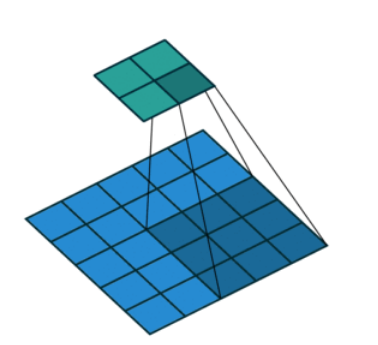
\includegraphics[width=.7\linewidth]{images/reg_conv}
  			\caption{}
  			\label{Fig:tranconva}
		\end{subfigure}
		\begin{subfigure}{.45\textwidth}
  			\centering
  			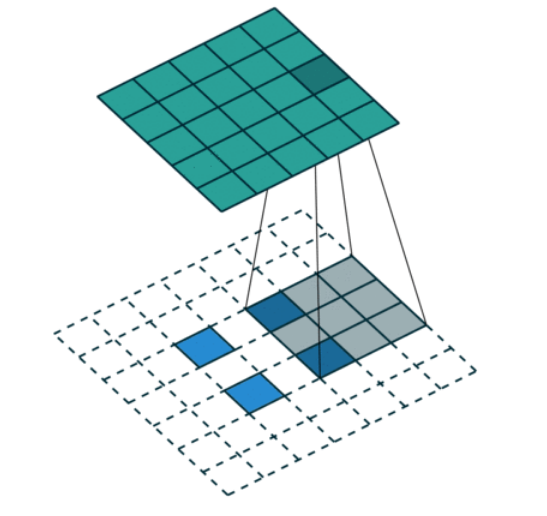
\includegraphics[width=.7\linewidth]{images/tran_conv}
  			\caption{}
  			\label{Fig:tranconvb}
		\end{subfigure}
		\caption{(a) 3$\times$3 convolution with stride 2 on a 5$\times$5 feature map (shown in blue) producing a 2$\times$2 feature map (shown in green). (b) 3$\times$3 fractionally strided convolution upsampling a 2$\times$2 feature map (shown in blue) to get a 5$\times$5 feature map (shown in green) \cite{diff_conv}.}
		\label{Fig:tranconv}
	\end{figure}

After replacing the fully-connected layers with convolutional layers, we are left with 3D feature maps with reduced spatial size. These 3D feature maps need to be upsampled back to the original input spatial size. One way to do this is to use an interpolation method such as bilinear interpolation to increase the spatial resolution. This is considered as a naive method of upsampling. An alternative would be to use fractionally strided convolutions (also known as transpose convolution or deconvolution). This type of convolution as shown in Figure \ref{Fig:tranconvb}, pads zeros to the input feature map in a manner which results in the desired upsampling when convolved over. In this example, we see a 2$\times$2 feature map upsampled to 5$\times$5 feature map by adding a row and a column of zeros in between the two existing rows and columns respectively and also zero padding by 2 around the feature map. A 3$\times$3 convolution can now be used to get back a spatial size of 5$\times$5. The advantage of using a fractionally strided convolution is that the parameters of the filter are learned through training instead of using a fixed upsampling method such as interpolation.
